\documentclass[noheader]{coursclass}

\usetikzlibrary{calc,positioning}

\begin{document}

\vspace*{-1.5cm}
\begin{definition}[Arbre de probabilités]
	Une expérience aléatoire peut être représentée par un \textbf{arbre de probabilités} si elle est composée de plusieurs \textit{épreuves}.

	Deux épreuves sont \textbf{indépendantes} lorsque le résultat de l'une n'influence pas la probabilité des résultats de l'autre.
\end{definition}

\begin{exemple}
	\begin{minipage}{0.5\linewidth}
		On fait une expérience qui consiste à lancer un dé équilibré 3 fois de suite, et à regarder si on a obtenu un $6$.

		On note $A$ l'évènement «Le dé est tombé sur $6$». Ainsi on peut dessiner l'arbre suivant :
	\end{minipage}
	\begin{minipage}{0.45\linewidth}
		\begin{center}
			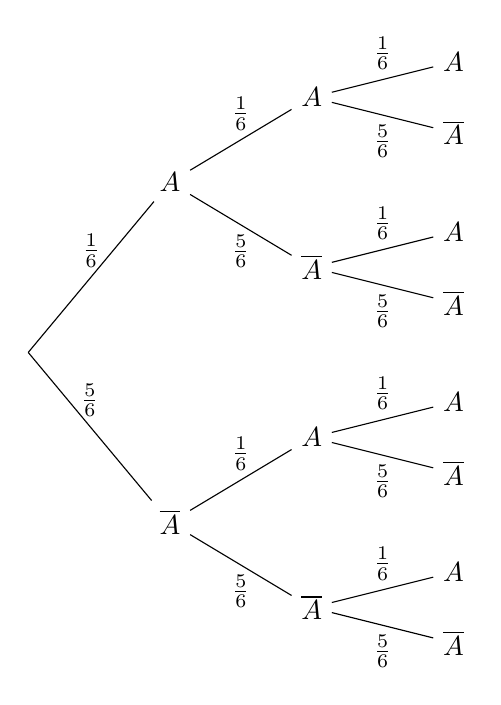
\begin{tikzpicture}[scale=0.9]
				\coordinate (START) at (0,0);
				\node (A) at (2,2.4) {$A$};
				\node (NA) at (2,-2.4) {$\overline{A}$};
				\draw (START) -- node[above] {$\frac{1}{6}$} (A)
				(START) -- node[above] {$\frac{5}{6}$} (NA);
				\foreach \n in {A,NA} {
						\node (Ab) at ($(\n) + (2,1.2)$) {$A$};
						\node (NAb) at ($(\n) + (2,-1.2)$) {$\overline{A}$};
						\draw (\n) -- node[above] {$\frac{1}{6}$} (Ab);
						\draw (\n) -- node[below] {$\frac{5}{6}$} (NAb);
						\foreach \nb in {Ab,NAb} {
								\node (Ac) at ($(\nb) + (2,0.5)$) {$A$};
								\node (NAc) at ($(\nb) + (2,-0.5)$) {$\overline{A}$};
								\draw (\nb) -- node[above] {$\frac{1}{6}$} (Ac);
								\draw (\nb) -- node[below] {$\frac{5}{6}$} (NAc);
							}
					}
			\end{tikzpicture}
		\end{center}
	\end{minipage}
\end{exemple}

\begin{exemple}
	Si on veut obtenir la probabilité d'obtenir \textit{exactement} $1$ six sur les trois lancés :

	Cet évènement est constitué des issues $\correctionDots{(A, \overline{A}, \overline{A})}$, $\correctionDots{(\overline{A}, A, \overline{A})}$ et $\correctionDots{(\overline{A}, \overline{A}, A)}$. Sa probabilité est donc

	\begin{center}
		\begin{tikzpicture}
			\coordinate (START) at (0,0);
			\node (A) at (2,2.4) {$A$};
			\node (NA) at (2,-2.4) {$\overline{A}$};
			\draw (START) -- node[above] {$\frac{1}{6}$} (A)
			(START) -- node[above] {$\frac{5}{6}$} (NA);
			\foreach \n in {A,NA} {
					\node (Ab) at ($(\n) + (2,1.2)$) {$A$};
					\node (NAb) at ($(\n) + (2,-1.2)$) {$\overline{A}$};
					\draw (\n) -- node[above] {$\frac{1}{6}$} (Ab);
					\draw (\n) -- node[below] {$\frac{5}{6}$} (NAb);
					\foreach \nb in {Ab,NAb} {
							\node (Ac) at ($(\nb) + (2,0.5)$) {$A$};
							\node (NAc) at ($(\nb) + (2,-0.5)$) {$\overline{A}$};
							\draw (\nb) -- node[above] {$\frac{1}{6}$} (Ac);
							\draw (\nb) -- node[below] {$\frac{5}{6}$} (NAc);
						}
				}
			\coordinate (TEMP) at (6,0.7);
			\node[right=of TEMP] {\correction{→ issue $(A, \overline{A}, \overline{A})$, probabilité $\dfrac{1}{6} × \dfrac{5}{6} × \dfrac{5}{6} = \dfrac{25}{216}$}};
			\coordinate (TEMP) at (6,-1.9);
			\node[right=of TEMP] {\correction{→ issue $(\overline{A}, A, \overline{A})$, probabilité $\dfrac{5}{6} × \dfrac{1}{6} × \dfrac{5}{6} = \dfrac{25}{216}$}};
			\coordinate (TEMP) at (6,-3.3);
			\node[right=of TEMP] {\correction{→ issue $(\overline{A}, \overline{A}, A)$, probabilité $\dfrac{5}{6} × \dfrac{5}{6} × \dfrac{1}{6} = \dfrac{25}{216}$}};
		\end{tikzpicture}

		$$ \correction{\dfrac{25}{216} + \dfrac{25}{216} + \dfrac{25}{216} = \dfrac{75}{216} = \dfrac{25}{72}} $$
	\end{center}
\end{exemple}

\end{document}